\documentclass{article}
\usepackage[utf8]{inputenc}
\usepackage[T1]{fontenc}
\usepackage{graphicx}
\usepackage{hyperref}
\usepackage{geometry}
\geometry{margin=1in}

\title{CABIN}
\date{Encyclopaedia Britannica (1771)}

\begin{document}
\maketitle

\section*{Historical source}
\textbf{Entry ID:} \texttt{entry-cabin-2464} \\
\textbf{Volume ID:} 144133902 \\
\textbf{Character Count:} 330

\subsection*{Extracted Text}
CABIN, in the fea-language, a final room, or apartment, whereby there are a great many in fewelful parts of a flip, particularly on the quarter-deck, and on each side of the fleerage, for the officers of the flip to lie in.

The great cabin is the chief of ’all, and that which properly belongs to the captain, or chief commander.



\section*{Source record}
\begin{itemize}
\item \textbf{Dataset:} \texttt{NationalLibraryOfScotland/encyclopaedia\_britannica\_illustrated}
\item \textbf{Dataset Revision:} \texttt{309f765b1ecc83e0a7f7762e44b4a927a7555443}
\item \textbf{Page ID:} \texttt{britannica:309f765b1ecc83e0a7f7762e44b4a927a7555443:train:2464} \\
  \textbf{Filename:} \texttt{page-2464-24f450326eee.jpg} \\
  \textbf{Row Index:} 2464 \\
  \textbf{SHA256:} \texttt{24f450326eee13b0...}
\end{itemize}

\begin{figure}[h]
\centering
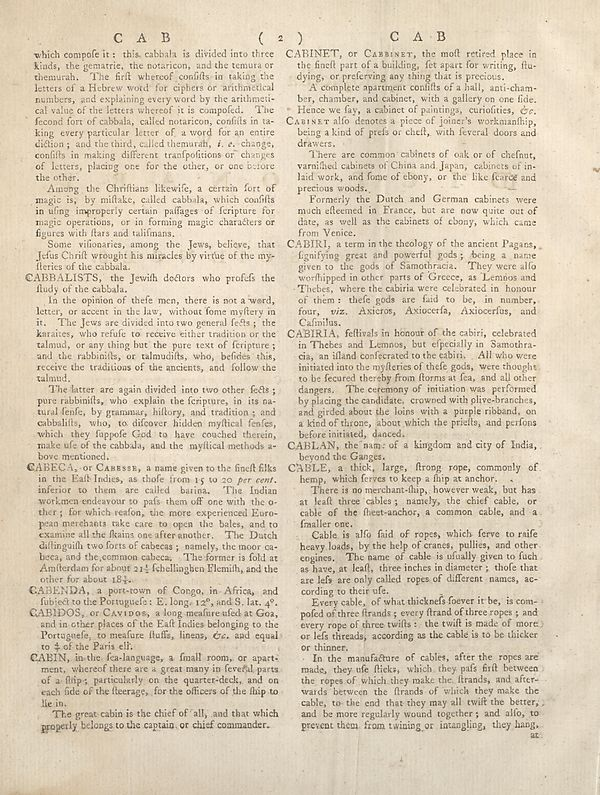
\includegraphics[width=0.85\textwidth]{../scans/page-2464-24f450326eee.jpg}
\caption*{Source scan: \texttt{page-2464-24f450326eee.jpg}}
\end{figure}

\end{document}
